\begin{figure}
\centering
\begin{tikzpicture}
  \node[inner sep=0pt] (circuit) at (0,0) {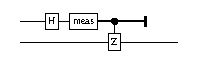
\includegraphics[scale=2]{Figures/circuits/disentangler}};
  \coordinate[below left=10.7mm and 0mm of circuit.north west] (leftPoint);
  \coordinate[right=61mm of leftPoint] (rightPoint);
  \pic (cut) {cut=leftPoint/rightPoint};
  \node[font=\scriptsize\itshape, opacity=0.9, above right=3mm and -3mm of leftPoint] (QPUA) {QPU A};
  \node[font=\scriptsize\itshape, opacity=0.9, below right=3mm and -3mm of leftPoint] (QPUB) {QPU B};
\end{tikzpicture}
\caption{Implementation of the cat-disentangler. Essentially, it destroys the ebit half (top wire) that the cat-entangler coupled with QPU B's wire. A doubled line indicates the wire holds classical information (a bit). For any input state \(\alpha\ket{0,0} + \beta\ket{1,1}\), the output is \(\alpha\ket{0} + \beta\ket{1}\).}
\label{fig:cat-disentangler}
\end{figure}